\documentclass[xcolor=dvipsnames]{beamer} 
\usetheme{Madrid}
\usepackage{booktabs}
\usepackage[T1]{fontenc}
\usepackage{pifont}
\usepackage{setspace}% http://ctan.org/pkg/setspace
\let\oldframetitle\frametitle% Store old \frametitle in \oldframetitle
\renewcommand{\frametitle}[1]{% Redefine \frametitle
	\oldframetitle{#1}\setstretch{1.25}}
\usepackage{natbib}
\bibpunct{(}{)}{;}{a}{}{,}
\usefonttheme{serif}
\usefonttheme{professionalfonts}
\usepackage{amsmath, tgpagella, eulerpx, eucal, hyperref, bookmark}
\useoutertheme{miniframes} 
\useinnertheme{circles}
\definecolor{darkred}{rgb}{0.55, 0.0, 0.0}
\usecolortheme[named=darkred]{structure} % you can change colortheme here

\title[Decolonization and the Global South]{Decolonization and the Global South}
\date{\today}
\author[Sanghoon Park]{Sanghoon Park \newline \newline  \footnotesize{Ph.D. Student}}
\institute[UofSC]{Department of Political Science}
\titlegraphic{
\includegraphics[width=4cm]{UofSC_Primary_RGB_G}}
\begin{document}
	
	\begin{frame}
		\titlepage
	\end{frame}
	\begin{frame}
		\tableofcontents
	\end{frame}
	
	\section{Introduction}
	\subsection{Teaching Assistant}
	\begin{frame}[fragile]{Who is your TA?}
		\begin{columns}[T]
			\begin{column}{0.36\textwidth}
				
\includegraphics[width=1\linewidth]{avatar.jpg}
			\end{column}
			
			\begin{column}{0.6\textwidth}
				\begin{itemize}
					\item \href{shpark.netlify.app}{Sanghoon Park}
					\item \href{sp23@email.sc.edu}{sp23@email.sc.edu}
					\item Office Hours
					\begin{itemize}
						\item \texttt{Mon} 11 am - 12 pm / \texttt{Tue} 1 - 2 pm
						\item You can make appointment: \href{https://calendly.com/sanghoon}{\texttt{Here}}
					\end{itemize}
					\item Research Interests
					\begin{itemize} 
						\item Authoritarian regimes
						\item Democratization
						\item Regime breakdown
					\end{itemize}
				\end{itemize}
			\end{column}
		\end{columns}
	\end{frame}
	
	\begin{frame}[fragile]{Office Hours: calendly.com/sanghoon}
		\begin{center}	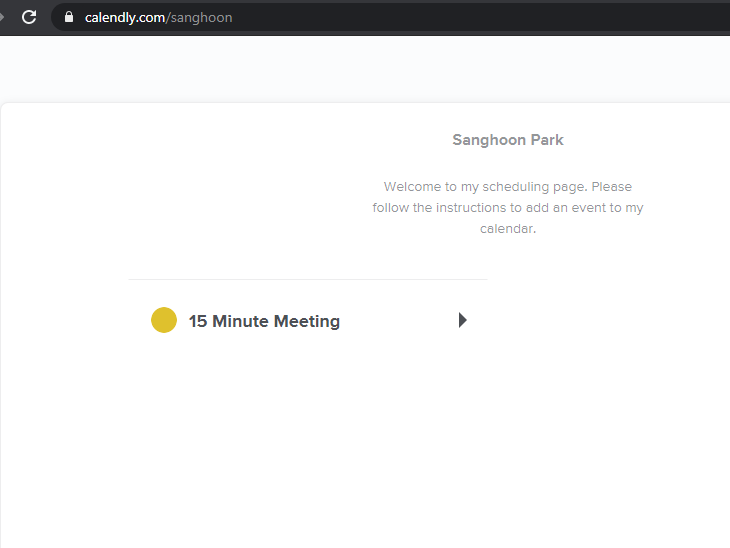
\includegraphics[width=0.7\linewidth]{officehours1.png} \end{center}
	\end{frame}
	
	\begin{frame}[fragile]{Office Hours: calendly.com/sanghoon}
		\begin{center}	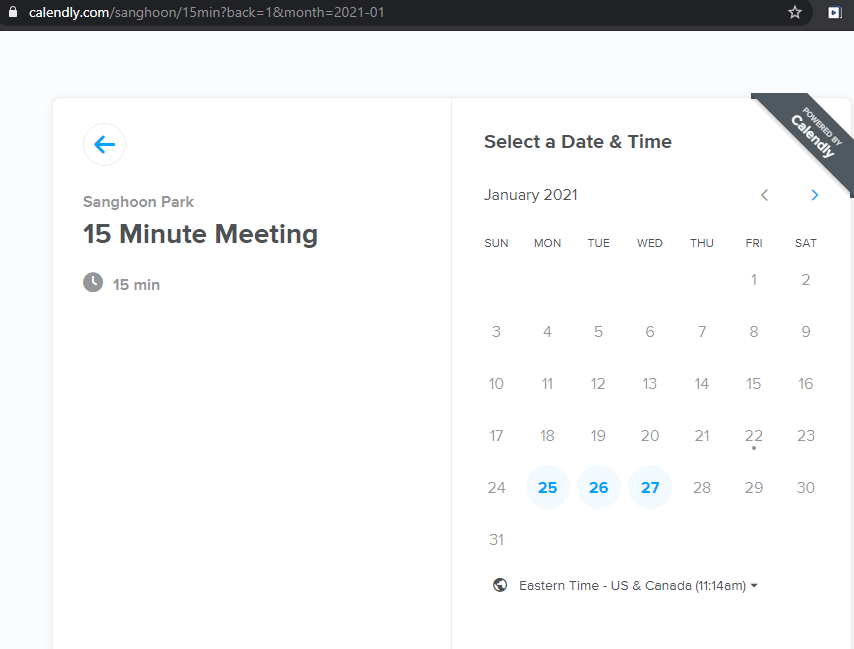
\includegraphics[width=0.7\linewidth]{officehours2.png}	\end{center}
	\end{frame}
	
	\begin{frame}[fragile]{Who is your TA?}
		\begin{columns}[T]
			\begin{column}{0.36\textwidth}
				
\includegraphics[width=1\linewidth]{avatar.jpg}
			\end{column}
			
			\begin{column}{0.6\textwidth}
				\begin{itemize}
					\item \href{shpark.netlify.app}{Sanghoon Park}
					\item \href{sp23@email.sc.edu}{sp23@email.sc.edu}
					\item Office Hours
					\begin{itemize}
						\item \texttt{Mon} 11 am - 12 pm / \texttt{Tue} 1 - 2 pm
						\item You can make appointment: \href{https://calendly.com/sanghoon}{\texttt{Here}}
					\end{itemize}
					\item Research Interests
					\begin{itemize} 
						\item Authoritarian regimes
						\item Democratization
						\item Regime breakdown
					\end{itemize}
				\end{itemize}
			\end{column}
		\end{columns}
	\end{frame}
	
	
	%De Juan Paper slides
	\section{De Juan and Pierskalla 2017}
	\subsection{The Comparative Politics of Colonialism and Its Legacies: An Introduction}
	
	\begin{frame}[fragile]{General question}
		\begin{columns}[T]
			\begin{column}{0.4\textwidth}
				\includegraphics[width=1\linewidth]{DeJuan2017cover.png}
			\end{column}
			
			\begin{column}{0.56\textwidth}
				\begin{center}
					\textit{\textcolor{blue}{Question:}}\\ \pause
					\bigskip		
					What are the causes and consequences of colonial rule?
				\end{center}
			\end{column}
		\end{columns}
	\end{frame}
	
	\begin{frame}[fragile]{Theories}
		Existing explanations
		\begin{itemize}
			\item Impacts of colonial legacies on economic/political development
			\begin{itemize}
				\item \textit{Types} of colonies affect the outcomes after decolonization
				\item Different economic/political institutions, legal systems, and social factors
			\end{itemize}
		\end{itemize}
		However, most of the explanations focus on between-variations in effects of decolonization based on different colonizers. \pause
		\begin{itemize}
			\item[] \centering\textit{What should we do next?}
		\end{itemize}
		
	\end{frame}
	
	\begin{frame}[fragile]{Theories}
		\citet{DeJuan2017} argue that we need something more to understand colonialism and its legacies fully.
		\begin{itemize}
			\item Survey the previous literature in Comparative Politics on colonialism.
			\item Show how recent scholars develop their theoretical arguments.
		\end{itemize}
	\end{frame}
	
	\begin{frame}[fragile]{Theories}
		\begin{itemize}
			\item Four trends in recent studies
			\begin{enumerate}
				\item Internal dynamics of colonial rule: within-variations \pause
				\begin{itemize}
					\item Local context, colonial agents and its administrations. \pause
				\end{itemize}
				\item Non-institutional interventions and transmission mechanisms \pause
				\item The role of contextual conditions \pause
				\begin{itemize}
					\item Influence of pre-colonial conditions after decolonization \pause
				\end{itemize}
				\item Increased disaggregation of outcome, explanatory variables, and unit of analysis \pause
				\begin{itemize}
					\item Go narrower and narrower.
					\item Macro (system-, cross-country institutions-level) $\rightarrow$ micro-foundational
				\end{itemize}
			\end{enumerate}
		\end{itemize}
	\end{frame}
	
	% Gartzke and Rohner 2011
	
	\section{Gartzke and Rohner 2011}
	\subsection{The Political Economy of Imperialism, Decolonization, and Development}
	
	\begin{frame}[fragile]{General question}
		\begin{columns}[T]
			\begin{column}{0.4\textwidth}
				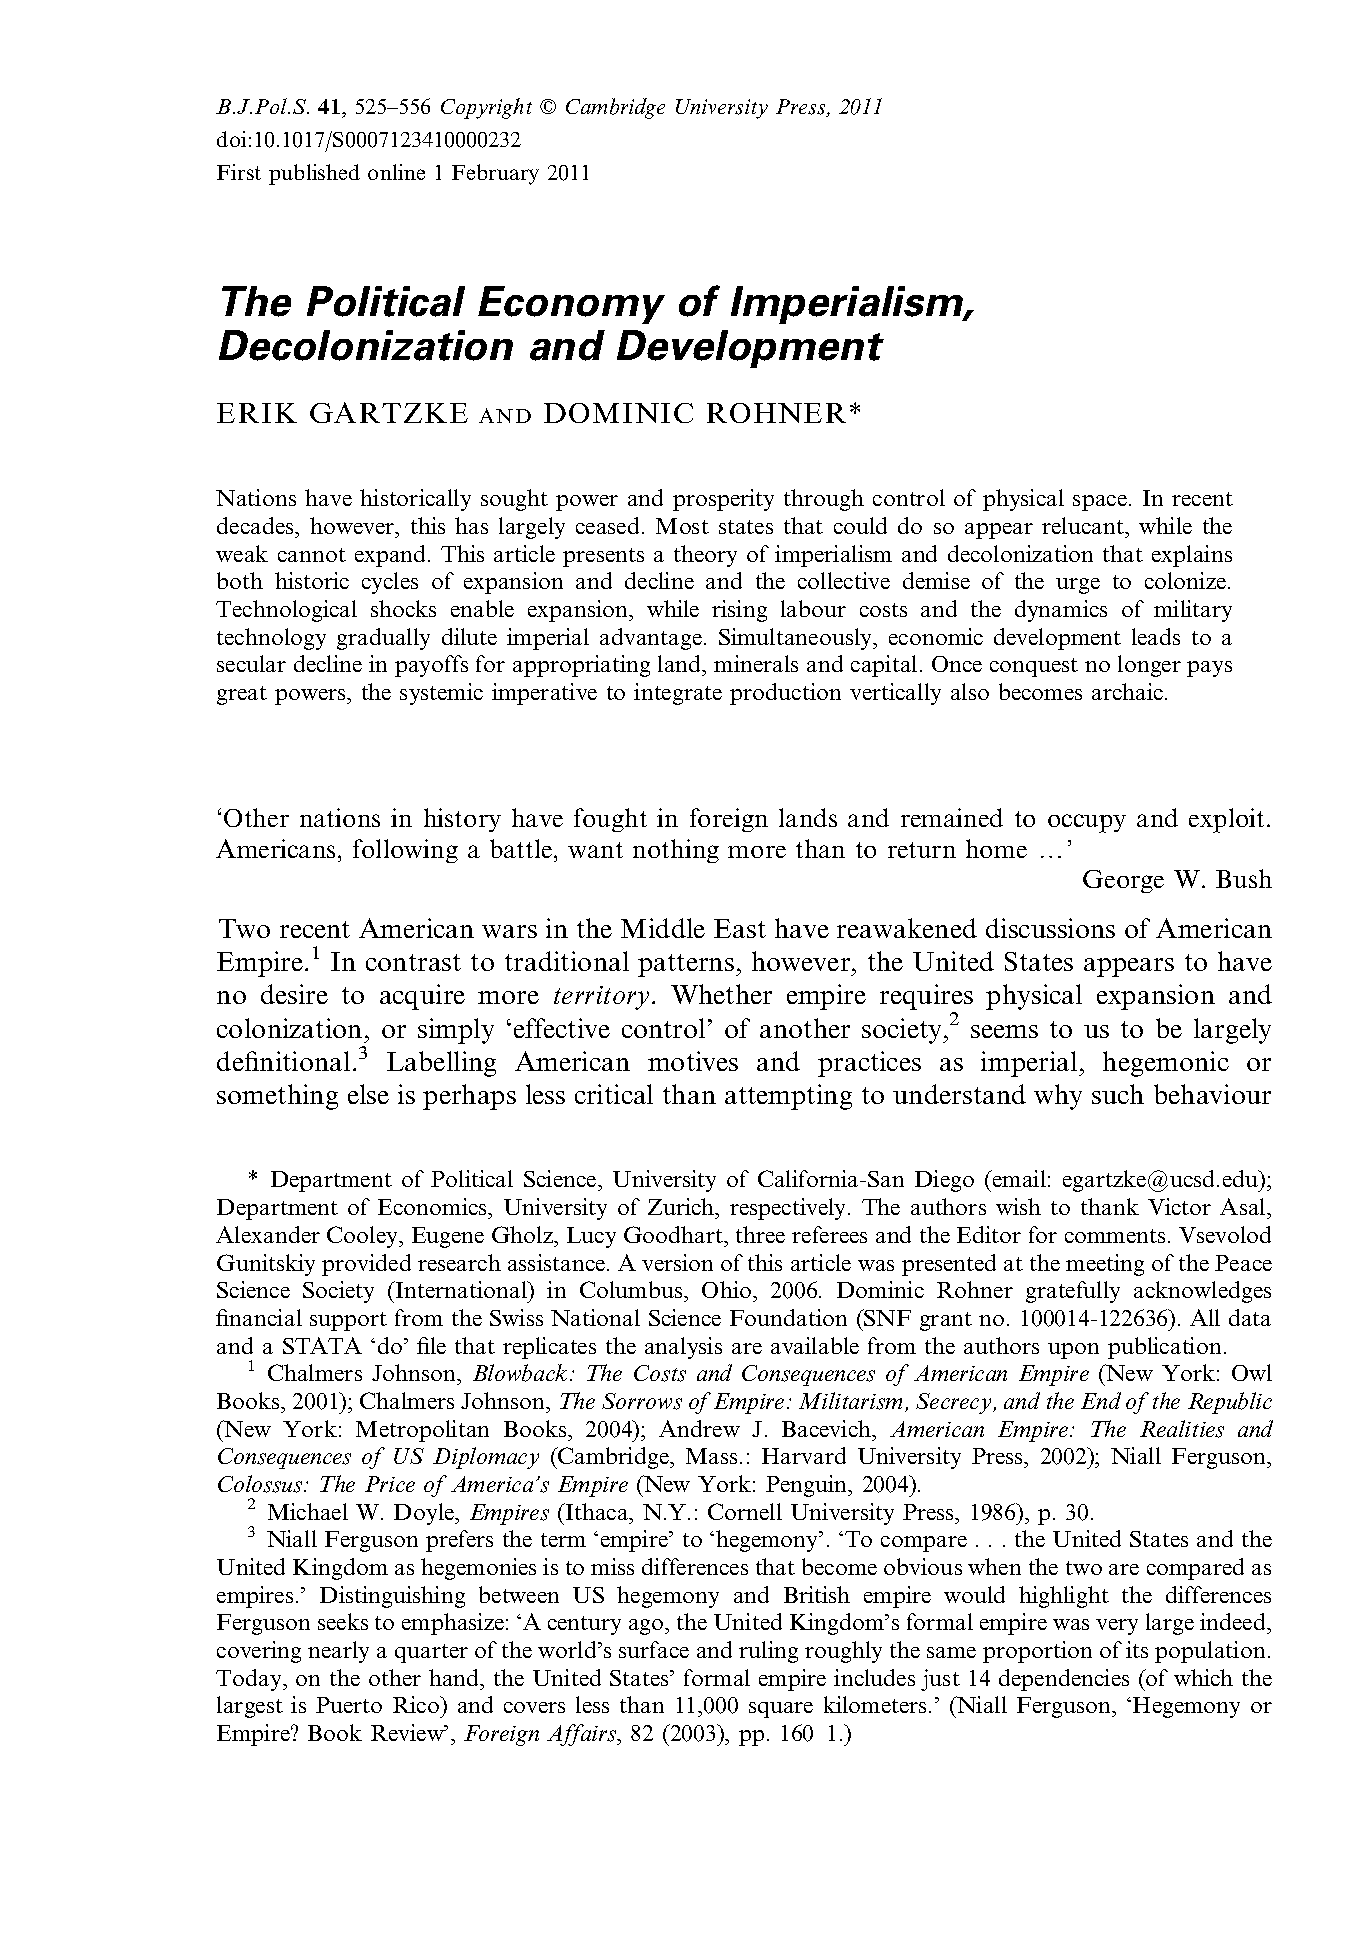
\includegraphics[width=1\linewidth]{Gartzke2011cover.png}
			\end{column}
			
			\begin{column}{0.56\textwidth}
				\begin{center}
					\textit{\textcolor{blue}{Question:}}\\ \pause
					\bigskip		
					What motivates an end of empire?\\ \pause
					\bigskip
					What makes empires (territorial expansions) unattractive now?
				\end{center}
			\end{column}
		\end{columns}
	\end{frame}
	
	\begin{frame}[fragile]{Theories}
		Existing explanations
		\begin{itemize}
			\item Imperialism: Find causes at Demand-side / Supply-side / System-level.
			\item Decolonization: Domestic politics in metropolis vs. International factors
		\end{itemize}
		\cite{Gartzke2011} point out that existing explanations can only explain one-way: \pause Rise (past) or Decline (present)  \pause
		\begin{itemize}
			\item[] \centering\textit{What should we do next?}
		\end{itemize}
		
	\end{frame}
	
	\begin{frame}[fragile]{Theories}
		\citet{Gartzke2011} offer a theory of imperialism and decolonization.
		\begin{itemize}
			\item Why \texttt{Military} < \texttt{Capital}? Why \texttt{Conquest} < \texttt{Commerce}?
		\end{itemize}\pause
		\citet{Gartzke2011} suggest micro-foundations for colonial expansion and decline. \pause
		\begin{enumerate}
			\item Military effectiveness
			\item Economic development $\rightarrow$ \textit{Imperialists' Dilemma}
		\end{enumerate}\pause
		Preference of territorial aggression is not given, but a variable driven by environmental conditions.\pause
		\begin{itemize}
			\item The preference can vary: decline and RECUR AGAIN.
		\end{itemize}
	\end{frame}
	
	\begin{frame}[fragile]{Models}
		\begin{center}
			When you read an article with scary models with\\\textit{Formula, Math symbols, or Greeks}.\pause
		\end{center}
		\begin{center}
			Read step-by-step.\\From the assumptions to their theoretical connections.\pause
		\end{center}
		\begin{center}
			Still scrary?\pause \\
			Find their implications that models want to say.\pause \\
			Here? Read \textit{\textbf{Hypotheses carefully.}}
		\end{center}
	\end{frame}
	
	\begin{frame}[fragile]{Models}
		General assumptions
		\begin{enumerate}
			\item Two actors
			\begin{itemize}
				\item $N$, $S$: Tribal groups, countries, or regions of the world.
				\item \citet{Gartzke2011} implicitly refer $N$ as colonizers, and $S$ as colonies in the models.
			\end{itemize}
		\end{enumerate}
	\end{frame}
	
	\begin{frame}[fragile]{Models}
		Let's try! \pause Really just try. \pause
		\begin{enumerate}[2]
			\item Production functions for each actor.
			\begin{equation*}
				\begin{aligned}
					y_{N}&= \alpha L^{a}_{N}K^{b}_{N}\\
					y_{S}&= \beta L^{c}_{S}K^{d}_{S}
				\end{aligned}
			\end{equation*}
			\begin{itemize}
				\item $y_{i}$ = production output for actor $i$
				\item $L_{i}$ = labor allocated to domestic production for actor $i$
				\item $K_{i}$ = physical capital and land stock for actor $i$
				\item $\alpha, \beta$ = total factor productivities
				\item $a, b, c, d$ = exogenous parameters
			\end{itemize}
		\end{enumerate}
	\end{frame}
	
	\begin{frame}[fragile]{Models}
		\begin{enumerate}[2]
			\item Production functions for each actor.
			\begin{itemize}
				\item We can change the previous-scary formula in plain words.
				\item $y_{N}= \alpha L^{a}_{N}K^{b}_{N}$
				\item "The production output for $N$ is determined by domestic labor allocations for $N$ \textbf{AND} physical capital and land stock for $N$, which depend on total factor productivity for $N$ ($\alpha$)."
				\item "Also, there exists external influences ($a, b$) on the labor allocations, physical capital, and land stocks in $N$."
			\end{itemize}
		\end{enumerate}
	\end{frame}
	
	\begin{frame}[fragile]{Models}
		Let's read the hypotheses (theoretical expectations)
		\begin{itemize}
			\item Colonialism and imperialism
			\begin{itemize}
				\item \textbf{\textit{$H_1$}}: Economic development $\cap$ Territorial Empire (concave)
				\item \textbf{\textit{$H_2$}}: Military effectiveness$\uparrow$ $\rightarrow$ Colonies $\uparrow$
				\item \textbf{\textit{$H_3$}}: Military tech$\uparrow$ $\rightarrow$ Colonies $\downarrow$
			\end{itemize}
			\item Political liberalization
			\begin{itemize}
				\item \textbf{\textit{$H_4$}}: Democracies $\rightarrow$ Colonies $\downarrow$
			\end{itemize}
			\item System effects
			\begin{itemize}
				\item \textbf{\textit{$H_5$}}: System contains many colonies $\rightarrow$ $\Pr$(Holding colonies)$\uparrow$
				\item \textbf{\textit{$H_6$}}: Hegemon has many colonies $\rightarrow$ $\Pr$(Holding colonies)$\uparrow$
				\item \textbf{\textit{$H_7$}}: System development $\cap$ $\Pr$(Holding colonies) (concave)
			\end{itemize}
		\end{itemize} 
	\end{frame}
	
	\begin{frame}[fragile]{Empirical results}
		Sample \pause $\rightarrow$ \textbf{IMPORTANT}
		\begin{itemize}
			\item Scope: Countries / Time: 1816-1992
			\item Unit of analysis: country-year (i.e. U.S. in 1816, U.S. in 1817)
		\end{itemize}
		Variables
		\begin{itemize}
			\item DV: Binary and counts of dependencies.
			\item EV: \textit{Economic development} / \textit{Fighting tech} / \textit{Democracy} / \textit{Fighting effectiveness} / \textit{Major power status} / \textit{Temporal dependence}
		\end{itemize}
		Methods \pause $\rightarrow$ \textbf{IMPORTANT, but not now}
		\begin{itemize}
			\item Negative binomial regression with robust standard errors.
		\end{itemize}
	\end{frame}
	
	\begin{frame}
		\begin{table}[ht]
			\small
			\centering
			\begin{tabular}[t]{lccc}
				\toprule
				EV						&Coeff.					&S.E.		&Expect		\\
				\midrule
				Economic Develp.		&1.909$^{***}$			&(0.399)	&  - 		\\
				Economic Develp.$^2$	&-0.183$^{***}$			&(0.046)	& Concave	\\
				Fighting Effectiveness	&41.17					&(24.40)	& Positive	\\
				Fighting Technology		&-69.01$^{***}$			&(18.68)	& Negative	\\
				Develp.$\times$Fight Tech&6.639$^{***}$			&(1.536)	& 			\\
				Democracy				&-0.0103				&(0.0649)	& Negative	\\
				Sys. Develp.			&12.35$^{***}$			&(3.424)	& - 		\\
				Sys. Develp.	$^2$	&-4.099$^{***}$			&(1.166)	& Concave	\\
				Hegemon (US)			&-2.317$^{***}$			&(0.585)	& Positive	\\
				Hegemon (US)$^2$		&0.168$^{***}$			&(0.042)	& Concave 	\\
				Major Power				&1.036					&(1.061)	& -  		\\
				\# States in System		&-0.0365*$^{**}$		&(0.011)	& -  		\\
				\# Major Powers			&0.345					&(0.186)	& - 		\\
				\bottomrule
			\end{tabular}
			\caption{The Political Economy of Decolonization}
		\end{table}
	\end{frame}
	
	
	\begin{frame}[fragile]{Conclusions}
		See \citet[555-556]{Gartzke2011}
		\begin{itemize}
			\item "The desire to control land$\cdots$remains strong in the developing world."
			\item "Successful development could increase middle tier, which is against territorial aggression."
			\item Tech. innovation$\uparrow$ $\rightarrow$ Labor costs $\uparrow$ = Costly empire
			\item However, decline of empire is not deterministic $\rightarrow$ It can recur or revive.
		\end{itemize}
	\end{frame}
	
	\section{Summaries}
	\begin{frame}[fragile]{Summaries}
		\cite{DeJuan2017}\pause
		\begin{itemize}
			\item Review previous literature on imperialism, colonialism.
			\item Suggest that we should look into micro-foundational dynamics.
			\item Good to skim: How are existing theories developed?.
		\end{itemize}\pause
		\cite{Gartzke2011}\pause
		\begin{itemize}
			\item I know...
			\item However, it addresses micro-foundations of imperialism, decolonization, and development.
			\item "Decolonialism" by strategic actors with varying preferences.
			\item Maybe a good practice if you read step-by-step.
		\end{itemize}
	\end{frame}
	
	\begin{frame}[fragile]{Questions}
		\begin{center}
			{\huge Thank you!}\\
			\bigskip		
			Any questions or meetings?\\
		\end{center}
		\begin{equation*}
			\begin{aligned}
				\text{\ding{43}}& \text{Email: \href{sp23@email.sc.edu}{sp23@email.sc.edu}}\\
				\text{\ding{43}}& \text{Calendly: \href{https://calendly.com/sanghoon}{\texttt{Here}}}
			\end{aligned}
		\end{equation*}
	\end{frame}
	
	\begin{frame}[t, fragile, allowframebreaks]{}
		\bibliographystyle{apsr}
		\bibliography{rd2.bib}
	\end{frame}
\end{document}